%----------------------------------------------------------------------------------------
%	PACKAGES AND OTHER DOCUMENT CONFIGURATIONS
%----------------------------------------------------------------------------------------

\documentclass{beamer}
%\usepackage{xcolor}
\usepackage{listings}
%\input{structure.tex} % Include the file specifying the document structure and custom commands

\usetheme{Frankfurt}

%----------------------------------------------------------------------------------------
%	ASSIGNMENT INFORMATION
%----------------------------------------------------------------------------------------

\title{The impact of agent definitions and interactions on multiagent learning for coordination} % Title of the assignment

\author{Authors: Jen Jen Chung, Damjan Miklić, Lorenzo Sabattini, Kagan Tumer, Roland Siegwart
\\ Presentors: Kallinteris Andreas, Orfanoudakis Stavros}

\date{13-2-2019} % University, school and/or department name(s) and a date

%----------------------------------------------------------------------------------------

\begin{document}
	\begin{frame}
		\maketitle % Print the title
	\end{frame}

	\section{Intro}
	\begin{frame}
		Domains with easily flexible agent defintions:
		\begin{itemize}
			\item Autonomus Traffic Management
			\item Network Routing
			\item Powerplant Control
		\end{itemize}
	\end{frame}
	\section{Domain}
	\begin{frame}
		\frametitle{Traffic Managment Domain}
		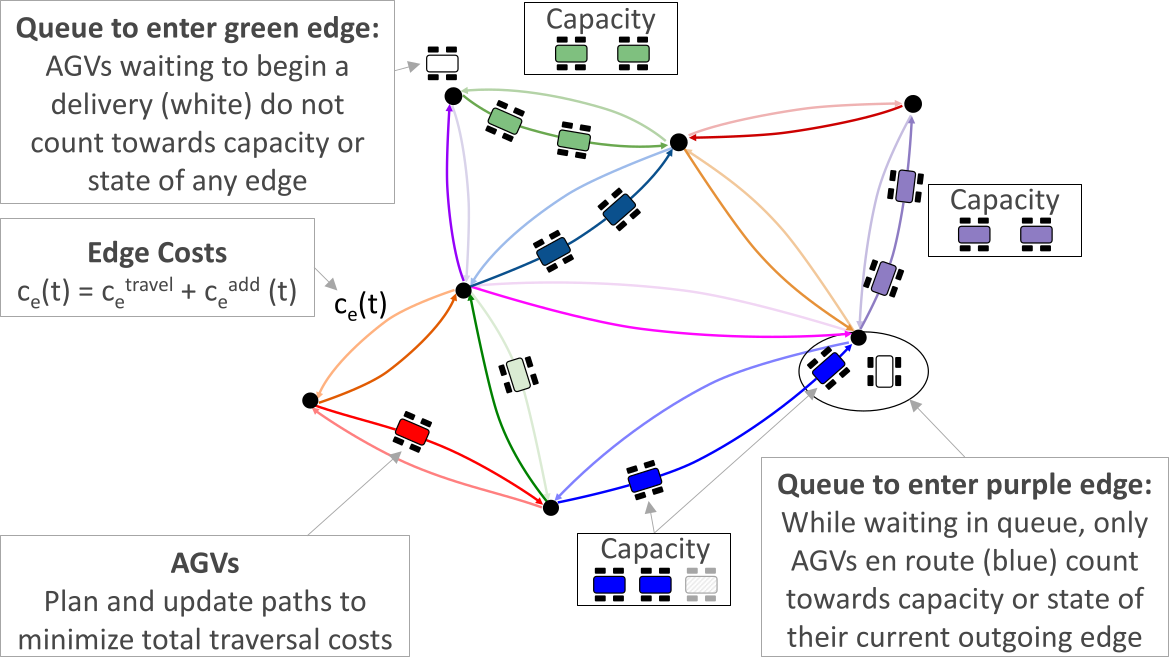
\includegraphics[width=\textwidth]{enviroment.png}
	\end{frame}
	\begin{frame}
		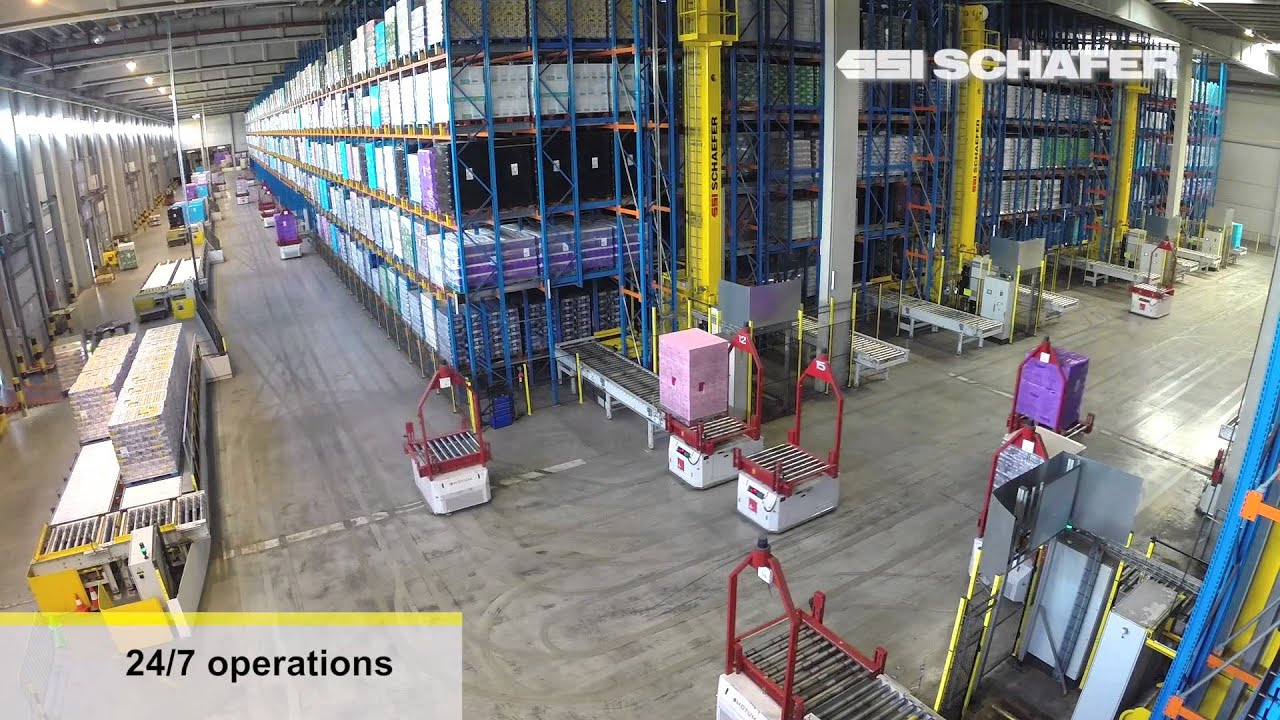
\includegraphics[width=\textwidth]{warehouse.jpg}
	\end{frame}
	\begin{frame}
		\frametitle{Variables}
		Cost for a AGV for traversing an edge
		\begin{itemize}
			\item $cost_e(t) = cost_e^{travel} + cost_e^{add}$
		\end{itemize}
		The Capacity of an edge (based on the physical space)
		\begin{itemize}
			\item $cap_e$
		\end{itemize}
	\end{frame}

	\section{Agent Defintion}
	\begin{frame}

	\end{frame}


\end{document}
